\chapter{Q Feed-Forward}
\label{ch:qff}

The motion model of the tracker, introduced in Section~\ref{subsec:tt_cca}, assumes that
the opponent moves with constant curvature and constant longitudinal acceleration over
each prediction interval. This assumption holds well when the dynamics of the opponent
changes slowly, e.g.\ on a straight or in the middle of a corner, but it is violated at
the beginning and at the end of the maneuvers. When the opponent starts braking, or
passes from braking to traction, the acceleration changes abruptly, and the actual
motion departs from the one predicted by the CCA model. In these conditions, the dynamic
model is no longer correct and the quality of the estimate degrades. The filter relies on
the motion model more than it should, and it follows the new dynamics only after several
measurements have confirmed it, so that the estimate lags behind the true state of the
opponent.

This behavior is shown in Fig.~\ref{fig:qff_cca_baseline}, which compares the speed and the
acceleration estimated by the filter with the CCA model and the nominal process noise with the
ground truth over two braking maneuvers. At the onset of each braking, the estimated
acceleration departs from the ground truth with a delay of several tenths of a second, and the
lag accumulated in this interval is reflected on the speed, which is overestimated during the
braking and underestimated at its end.

\begin{figure}[H]
    \centering
    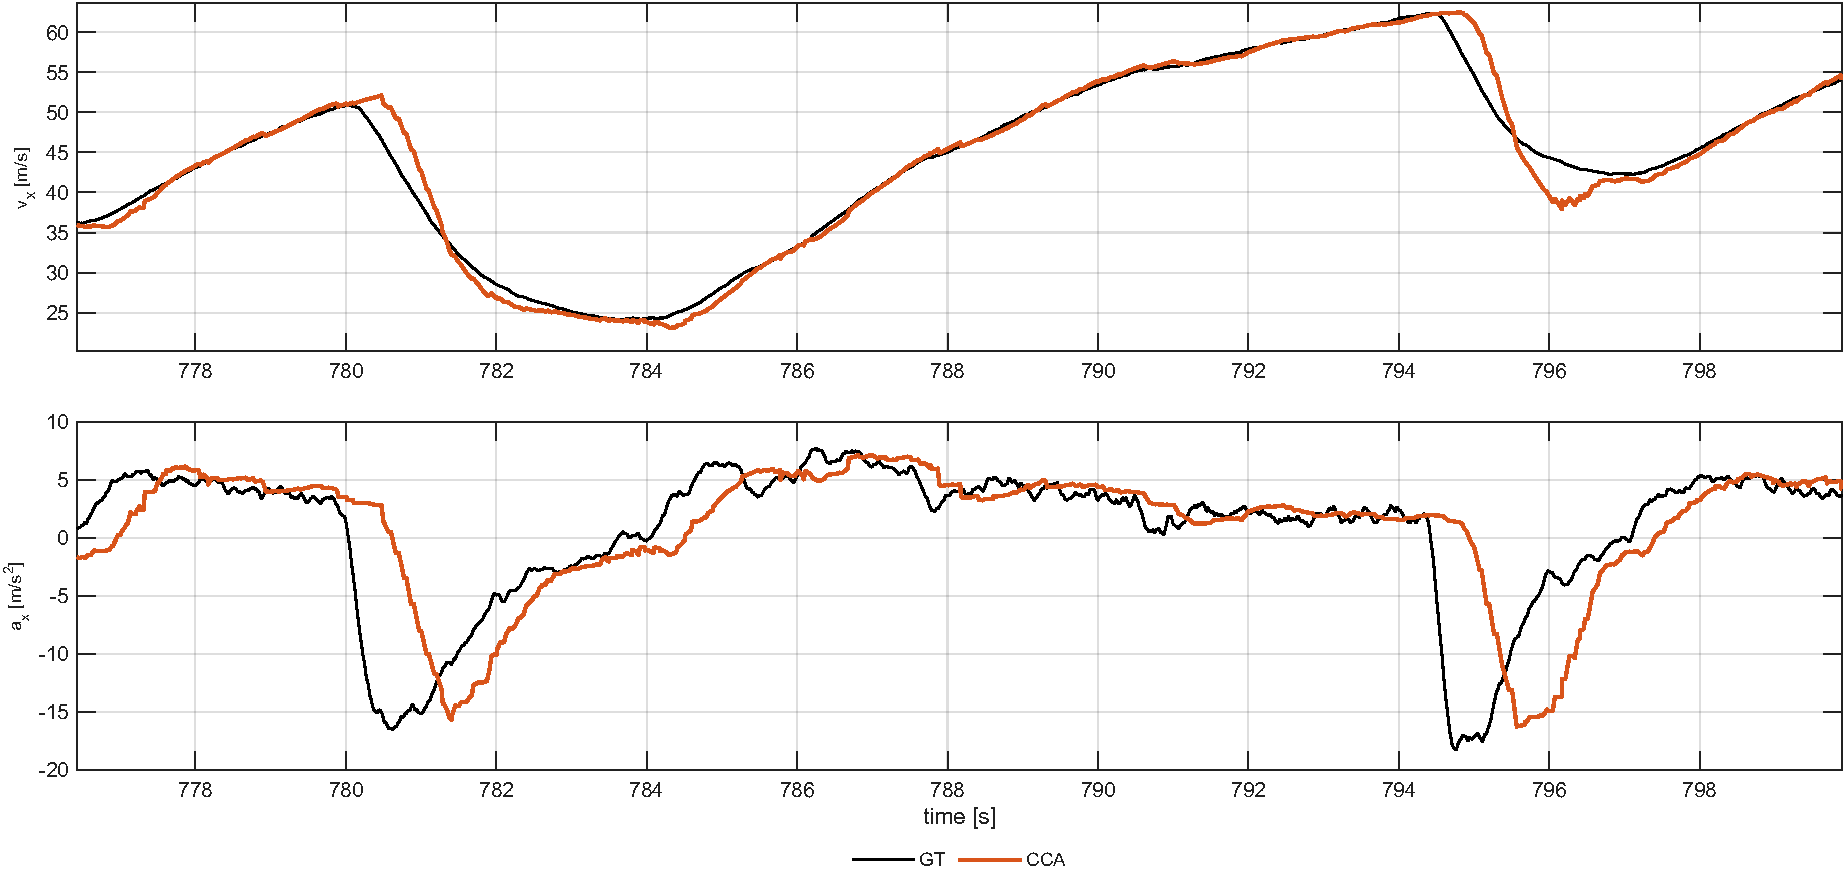
\includegraphics[width=0.8\textwidth]{figures/ch5/cca_baseline.pdf}
    \caption{Speed and acceleration estimated with the CCA model and the nominal process
    noise. Session of 5 September 2026, Imola.}
    \label{fig:qff_cca_baseline}
\end{figure}

Several approaches have been proposed to adapt a filter to the maneuvers of a target. A
first family adapts the process noise online from the innovations of the filter, as in the
covariance matching techniques, which estimate $\mathbf{Q}$ recursively from the discrepancy between the observed and the predicted dispersion of the
innovations, without requiring an explicit description of the maneuver. A second line of
research comprises the multiple model approaches, which estimate the state through several
filters running in parallel, each based on a motion model representative of an operating
condition of the vehicle. In the classical multiple model formulation, the filters evolve
independently and their estimates are only combined at the output, weighted by model
probabilities computed from the likelihood of the innovations. In the Interacting Multiple
Model (IMM) filter, instead, the filters also interact, since at each step their initial
conditions are obtained by mixing the estimates of all the models according to the
transition probabilities between them, which allows the estimate to follow the switches
between the operating conditions of the vehicle. These approaches describe the different
phases of the race with dedicated models, at the cost of a higher computational load, of a
larger number of parameters to tune, such as the transition probabilities between the
models, and of the need to mix states of different dimension. A further line, to which the
approach presented in this chapter belongs, is based on a maneuver detection logic, and it
lies between the previous two, since it starts from a single motion model but switches
between two distinct behaviors of the filter, with a nominal and an inflated process noise,
according to an explicit detection of the maneuver.

To recover the quality of the estimate during the maneuvers, a feed-forward approach on
the process noise covariance is therefore implemented. Its idea and rationale are explained in
Section~\ref{sec:qff_idea}, and Section~\ref{sec:qff_nominal} describes the preliminary tuning
of the nominal process noise, which is the starting value of the method.
Section~\ref{sec:qff_formulation} presents the feed-forward formulation, together with the
maneuver detection logic based on the jerk of the opponent and its implementation in the
tracker. Finally, Section~\ref{sec:qff_results} compares the resulting estimate with the one of
the nominal filter.

% =====================================================================
\section{The Idea}
\label{sec:qff_idea}

The idea behind the feed-forward approach presented in this chapter starts from how the
process noise covariance $\mathbf{Q}_k$ influences the gain of the Kalman filter. The
process noise represents the uncertainty of the motion model, i.e.\ how much the actual
motion of the opponent is expected to differ from the predicted one. In the prediction
step, it is added to the covariance propagated through the motion model,
\begin{equation}
    \mathbf{P}_{k+1|k} = \mathbf{F}_k\,\mathbf{P}_{k|k}\,\mathbf{F}_k^\top + \mathbf{Q}_k,
    \label{eq:qff_pred_cov}
\end{equation}
and the predicted covariance enters the Kalman gain of the correction step,
\begin{equation}
    \mathbf{K}_{k+1} = \mathbf{P}_{k+1|k}\,\mathbf{H}_{k+1}^\top
    \left(\mathbf{H}_{k+1}\,\mathbf{P}_{k+1|k}\,\mathbf{H}_{k+1}^\top + \mathbf{R}_{k+1}\right)^{-1},
    \label{eq:qff_gain}
\end{equation}
as in~\eqref{eq:tt_prediction} and~\eqref{eq:tt_update}. Considering a single component,
with a predicted variance $P$ and a measurement noise variance $R$, the gain reduces to
\begin{equation}
    K = \frac{P}{P + R},
    \label{eq:qff_gain_scalar}
\end{equation}
which ranges between zero, when the prediction is much more accurate than the
measurement, and one, when the measurement is much more accurate than the prediction.
Increasing $\mathbf{Q}_k$ increases $P$ and therefore $K$, so that the corrected state
moves away from the prediction and towards the measurement. Through the off-diagonal
terms of $\mathbf{P}_{k+1|k}$, the effect is not limited to the measured position. The
process noise of the CCA model acts on the acceleration and on the curvature
(Section~\ref{subsec:tt_cca}), and a larger uncertainty on these states allows the
correction of the position to be transferred more quickly to the speed and to the
acceleration, which are not measured directly by the LiDARs and by the camera.

By varying $\mathbf{Q}_k$, different behaviors of the filter are therefore obtained. A
large process noise leads to a large gain and therefore to a more reactive filter, which
follows the changes of the dynamics quickly but returns a noisy estimate. A small process
noise, instead, keeps the gain small, and the filter remains anchored to the prediction,
with a smoother estimate that is often delayed with respect to the true state.

\begin{figure}[H]
    \centering
    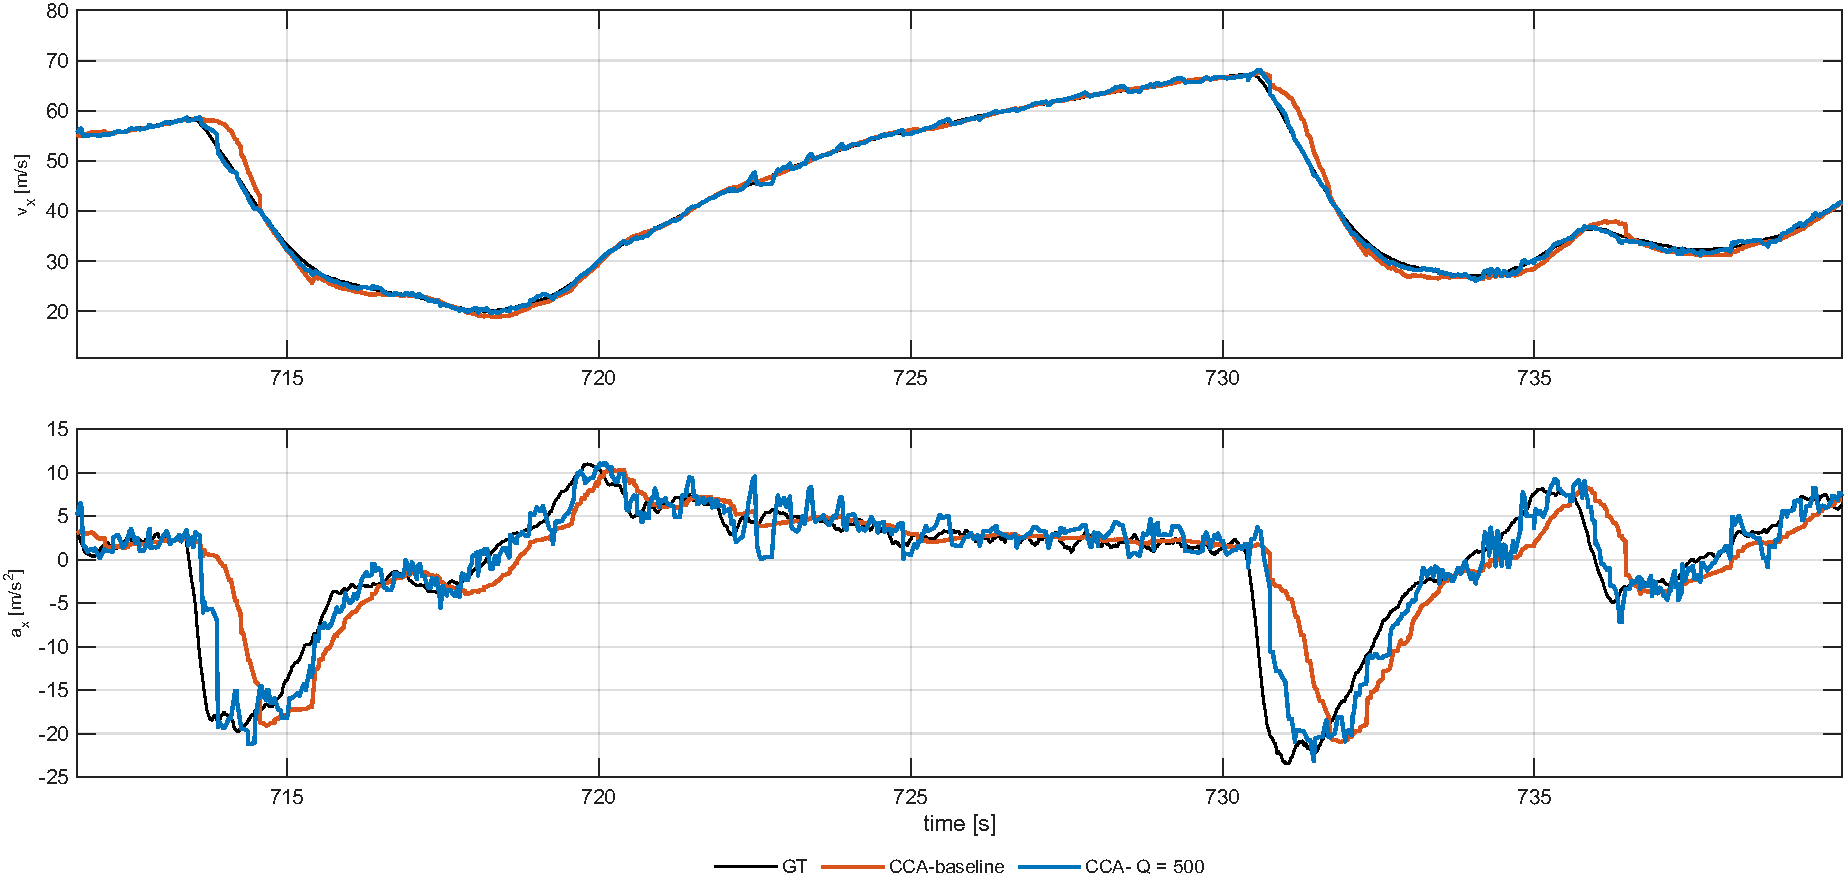
\includegraphics[width=\textwidth]{figures/ch5/q_high_vs_baseline.pdf}
    \caption{Speed and acceleration estimated with the nominal and with an increased process
    noise. Session of 5 September 2026, Imola.}
    \label{fig:qff_highq}
\end{figure}

Fig.~\ref{fig:qff_highq} shows the speed and the longitudinal acceleration of the opponent
estimated by the filter with the CCA model, with the nominal process noise and with an
increased one, obtained with $q_a = 500$, compared with the ground truth over two braking
maneuvers. The figure confirms the previous considerations. With the increased process noise,
the filter corrects the prediction more with the information of the measurements, and it is
therefore considerably more reactive at the changes of maneuver, with an acceleration that
closely follows the ground truth at the beginning and at the end of the braking phases. The
nominal filter, instead, follows the same transitions with a visible delay, which is also
reflected on the speed at the beginning of each braking.

Adopting the increased process noise over the whole lap, however, is not a correct solution,
since in the phases at constant acceleration the larger gain makes the filter follow the noise
of the measurements, and the estimate of the acceleration becomes noisier without any benefit,
as visible in Fig.~\ref{fig:qff_highq} between the two maneuvers. At the same time, a process
noise fixed at its nominal value cannot cover the whole spectrum of the dynamics of the
vehicle, which alternates slowly varying phases with abrupt transitions between traction and
braking. From these considerations arises the idea of the approach presented in this chapter,
i.e.\ to alternate between the two values of the process noise through a maneuver detection
logic, which in this work is implemented as a feed-forward approach and is presented in
Section~\ref{sec:qff_formulation}, after the tuning of the nominal process noise.

% =====================================================================
\section{Nominal Process Noise Tuning}
\label{sec:qff_nominal}

Preliminary to the feed-forward approach is the tuning of the nominal value
$\mathbf{Q}_{\mathrm{nom}}$ of the process noise, i.e.\ of the spectral densities $q_a$
and $q_\kappa$ of Section~\ref{subsec:tt_cca}. The choice is made by testing different
values of the process noise and selecting the one that gives a good starting point on the
trade-off introduced in the previous section, between the reactivity of the filter to
the changes of the dynamics and the noise of the estimate. This value is the baseline of
the feed-forward approach, in which it is multiplied by an inflation factor during the
maneuvers.

\TODO{Figures with the estimate obtained with different values of the process noise, and
their effect on the quality of the estimate.}

% =====================================================================
\section{Feed-Forward Formulation}
\label{sec:qff_formulation}

In the feed-forward formulation, the process noise covariance of the filter is switched
between two values, the nominal one, suited to the phases in which the dynamics of the
opponent changes slowly, and an inflated one, which makes the filter reactive during the
maneuvers. The switch is driven by a maneuver flag $f_k$, which is activated when a maneuver is
detected and deactivated when it is over,
\begin{equation}
    \mathbf{Q}_k =
    \begin{cases}
        \mathbf{Q}_{\mathrm{nom}} & \text{if } f_k = 0, \\
        \lambda\,\mathbf{Q}_{\mathrm{nom}} & \text{if } f_k = 1,
    \end{cases}
    \label{eq:qff_switch}
\end{equation}
where $\mathbf{Q}_{\mathrm{nom}}$ is the nominal process noise of
Section~\ref{sec:qff_nominal} and $\lambda > 1$ the inflation factor. The flag therefore
selects at each step which of the two behaviors of the filter is adopted, the reactive or the
nominal one, while the motion model and the structure of the filter remain unchanged.

The maneuver detection is based on the jerk of the opponent, i.e.\ the time derivative of its
longitudinal acceleration, which is the natural candidate for this purpose. The CCA model
assumes a constant acceleration over each prediction interval, and the jerk, being its
derivative, directly measures how much the actual motion departs from this assumption, so that
its magnitude is small in the phases that the model describes correctly and large at the
beginning and at the end of the maneuvers. The detection logic is described in
Section~\ref{subsec:qff_detection}, and its implementation in the tracker in
Section~\ref{subsec:qff_implementation}.

\subsection{Maneuver Detection Logic}
\label{subsec:qff_detection}

As anticipated in the previous section, the maneuver is detected from the instantaneous value
of the jerk of the opponent. Since the jerk is not measured by the sensors, it has to be
estimated, and two approaches are possible.

The first consists in augmenting the state of the filter with the jerk, which turns the CCA
model into a constant-jerk model, in which the jerk evolves as a random walk driven by a white
noise on its derivative. Besides requiring a new formulation of the motion model, of its
Jacobians and of the discretized process noise, whose terms would propagate to all the other
states, this solution is not pursued for two main reasons. The jerk would be observed only
indirectly, since it is separated by two integrations from the range rate of the RaDAR and by
three from the measured position, so that its estimate would be corrected only through the
cross-covariance terms of the filter, with a small gain and a convergence time comparable to
the duration of the maneuvers themselves, which contrasts with the need for an early
detection. Moreover, the additional state would modify the estimator published to the planning
module also where the CCA model is adequate, since a higher-order model amplifies the effect of
the measurement noise on the prediction, whereas the purpose of the detection is only to
select the process noise, leaving the nominal behavior of the filter unchanged outside the
maneuvers.

The second approach, adopted in this work, consists in obtaining the jerk by differentiating
and filtering the estimated acceleration. The filtering limits the amplification of the
high-frequency noise caused by the differentiation, and two families of filters are
considered, time-domain and frequency-based ones.

\paragraph{Time-domain filters.} In this family, the differentiated acceleration is
filtered by interpolating the signal with a polynomial of degree $n$ over a moving window
of $m$ samples. The degree of the polynomial sets the degrees of freedom of the fit,
while the length of the window sets the number of samples used for the fitting, and
therefore the amount of smoothing. The classical filter of this family is the
Savitzky--Golay filter. Polynomial filters, however, typically optimize the estimate at
the center of the window. In a real-time application, this would require using both the
past and the future samples of the signal, which are not available online. For this
reason, this family is discarded, and the frequency-based filters are adopted.

\paragraph{Frequency-based filters.} In this family, the acceleration is differentiated
and filtered with a low-pass filter. Both filters can be written as the product of the
derivative and of a low-pass filter $L(s)$,
\begin{equation}
    H(s) = s\,L(s).
    \label{eq:qff_diff}
\end{equation}
Among the filters considered is the first-order low-pass filter, which combined with the
derivative gives the dirty derivative, i.e.\ a differentiator band-limited by a pole with
time constant $\tau$,
\begin{equation}
    H_1(s) = \frac{s}{1 + \tau s}.
    \label{eq:qff_dirty}
\end{equation}
The second is the Butterworth filter of the second order, with cutoff frequency
$\omega_c$, whose combination with the derivative gives
\begin{equation}
    H_2(s) = \frac{s\,\omega_c^2}{s^2 + \sqrt{2}\,\omega_c\, s + \omega_c^2}.
    \label{eq:qff_butter}
\end{equation}
The Bode diagrams of the two transfer functions are shown in Fig.~\ref{fig:qff_bode}. Both
behave as a differentiator below the cutoff frequency, whereas above it $|H_1|$ tends to the
constant $1/\tau$ and $|H_2|$ decreases by \SI{20}{dB} per decade. Being of the second order,
the Butterworth filter therefore guarantees a better roll-off, i.e.\ a stronger attenuation of
the disturbances above the cutoff frequency, while keeping a flat pass band, and it is for this
reason adopted to estimate the jerk.

\begin{figure}[H]
    \centering
    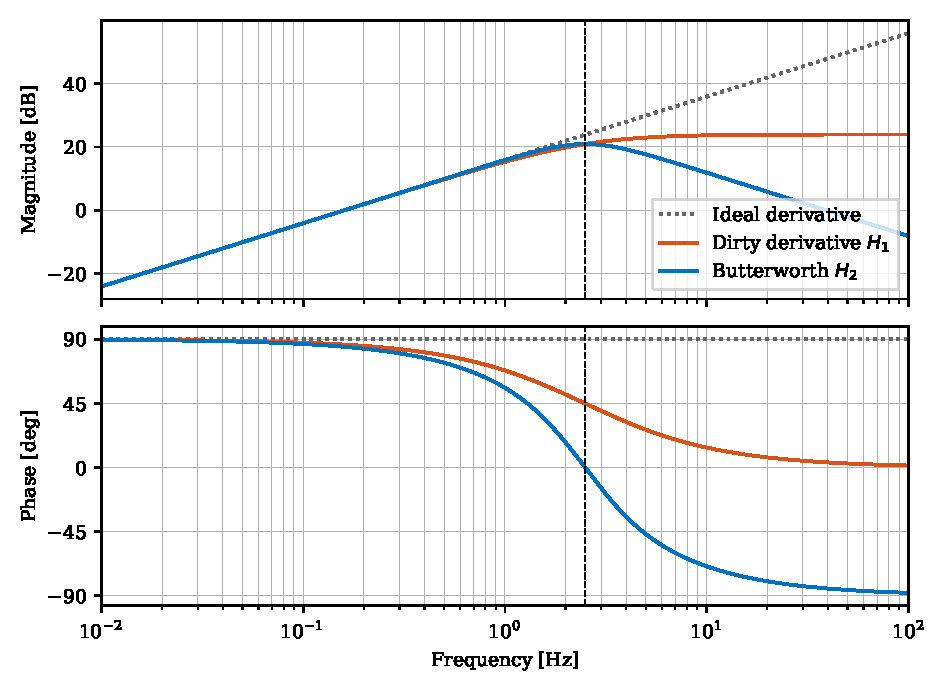
\includegraphics[width=0.85\textwidth]{figures/ch5/jerk_filters_bode.pdf}
    \caption{Bode diagrams of the dirty derivative $H_1$ and of the Butterworth filter $H_2$.}
    \label{fig:qff_bode}
\end{figure}

The activation thresholds of the flag are chosen by considering the jerk estimated from the
ground truth, by looking at its values when the vehicle is on a straight, i.e.\ with a slowly
varying dynamics, and when its dynamics changes, at the beginning and at the end of the
maneuvers, so that the latter exceed the upper threshold while the former remain mostly below
the lower one.

Once the jerk is estimated, the maneuver is detected through a hysteresis logic on its
magnitude, based on two thresholds $j_{\mathrm{on}} > j_{\mathrm{off}}$ and described by the
finite state machine of Fig.~\ref{fig:qff_fsm}. The flag is activated when the magnitude of the
jerk exceeds the upper threshold, and it is deactivated only when it falls below the lower
one. Between the two thresholds, the flag keeps its previous state, so that small oscillations
of the jerk around a single threshold do not switch it repeatedly, which limits the false
detections and the chattering of the flag.

\begin{figure}[H]
    \centering
    % Finite state machine of the maneuver flag (Chapter 5, feed-forward process noise).
\begin{tikzpicture}[
    font=\footnotesize,
    >={Stealth[length=2mm]},
    state/.style={circle, draw, thick, minimum size=21mm, align=center, font=\footnotesize},
    tr/.style={->, thick},
    lab/.style={font=\scriptsize, align=center, fill=white, inner sep=1.5pt}
]
\node[state, fill=black!5] (OFF) at (0,0) {\textbf{OFF}\\[2pt] $\mathbf{Q}_k = \mathbf{Q}_{\mathrm{nom}}$};
\node[state, fill=black!15] (ON) at (6,0) {\textbf{ON}\\[2pt] $\mathbf{Q}_k = \lambda\,\mathbf{Q}_{\mathrm{nom}}$};

% initial state
\coordinate (S) at (-2.6,0);
\fill (S) circle (2pt);
\draw[tr] (S) -- (OFF);

% transitions
\draw[tr] (OFF) to[bend left=22] node[lab, above]{$|j_k| > j_{\mathrm{on}}$} (ON);
\draw[tr] (ON) to[bend left=22] node[lab, below]{$|j_k| < j_{\mathrm{off}}$} (OFF);

% self loops
\draw[tr] (OFF) to[out=120, in=60, looseness=5] node[lab, above]{$|j_k| \le j_{\mathrm{on}}$} (OFF);
\draw[tr] (ON) to[out=120, in=60, looseness=5] node[lab, above]{$|j_k| \ge j_{\mathrm{off}}$} (ON);
\end{tikzpicture}

    \caption{Finite state machine of the maneuver flag.}
    \label{fig:qff_fsm}
\end{figure}

\subsection{Implementation}
\label{subsec:qff_implementation}
\label{sec:qff_implementation}

The main aspect of the implementation is the choice of the acceleration from which the jerk is
estimated. Deriving it from the filter whose process noise is switched would not allow the
maneuver to be detected in time. As shown in Fig.~\ref{fig:qff_highq}, with the nominal process
noise the acceleration follows the transitions with a delay, so that its derivative would
exceed the activation threshold only when the maneuver is already in progress, i.e.\ after the
delay that the method aims to reduce has been accumulated. The best estimate of the jerk is
instead obtained by differentiating the acceleration of the filter with the increased process
noise, which in Fig.~\ref{fig:qff_highq} is the closest to the ground truth at the changes of
maneuver, being the filter in its most reactive condition. Its larger noise is acceptable,
since this estimate is used only for the detection.

For this reason, the feed-forward approach is implemented with two filters that evolve in
parallel for each track and process the same measurements, according to the architecture of
Fig.~\ref{fig:qff_scheme}. The first is the main filter of Chapter~\ref{ch:tracking}, whose
process noise is switched by the hysteresis logic and whose state is published to the planning
module. The second, auxiliary, filter has the same structure, i.e.\ the EKF with the CCA model,
but its process noise is constant and increased, and it is used only to estimate the jerk and,
therefore, to drive the maneuver flag.

The auxiliary filter also avoids a coupling between the flag and the estimate. If the jerk were
derived from the main filter, the activation of the flag would inflate the process noise of
the same filter, making its acceleration noisier and its jerk larger, which would in turn keep
the flag active. The detection would then depend on its own output, in a feedback loop. Since
the process noise of the auxiliary filter does not depend on the flag, the detection is
decoupled from the switching, and the process noise of the main filter is set in feed-forward.

\begin{figure}[H]
    \centering
    % Architecture of the feed-forward process noise (Chapter 5).
\begin{tikzpicture}[
    font=\footnotesize,
    >={Stealth[length=2mm]},
    blk/.style={draw, thick, rounded corners=2pt, minimum width=22mm, minimum height=10mm, align=center},
    aux/.style={blk, fill=black!5},
    main/.style={blk, fill=black!15},
    arr/.style={->, thick},
    lab/.style={font=\scriptsize, align=center, fill=white, inner sep=1.2pt}
]
\node (Z) at (0,-1.4) {$\mathbf{z}_k$};
\coordinate (S) at (1.2,-1.4);
\node[aux]  (A) at (3.2,0)    {Auxiliary EKF\\ inflated $\mathbf{Q}$};
\node[aux]  (J) at (6.6,0)    {Jerk\\ estimation};
\node[aux]  (H) at (10,0)     {Hysteresis\\ logic};
\node[blk]  (Q) at (10,-2.8)  {Process noise\\ switch};
\node[main] (M) at (3.2,-2.8) {Main EKF\\ $\mathbf{Q}_k$};
\node (P) at (3.2,-4.6) {state published to the planning module};
\draw[thick] (Z) -- (S);
\draw[arr] (S) |- (A.west);
\draw[arr] (S) |- (M.west);
\draw[arr] (A) -- node[lab,above]{$a_k$} (J);
\draw[arr] (J) -- node[lab,above]{$j_k$} (H);
\draw[arr] (H) -- node[lab,right]{$f_k$} (Q);
\draw[arr] (Q) -- node[lab,above]{$\mathbf{Q}_{\mathrm{nom}}$ or $\lambda\mathbf{Q}_{\mathrm{nom}}$} (M);
\draw[arr] (M) -- (P);
\fill (S) circle (1.5pt);
\end{tikzpicture}

    \caption{Architecture of the feed-forward process noise.}
    \label{fig:qff_scheme}
\end{figure}

The jerk is estimated only on the updates that include the range rate of the RaDAR. Without it,
the acceleration of the auxiliary filter is corrected only through the position measurements,
which are separated from the jerk by three successive differentiations, so that the
corrections of the position would be strongly amplified in the jerk and would lead to false
activations of the flag. The jerk is estimated with the second-order Butterworth
filter~\eqref{eq:qff_butter}, the thresholds of the hysteresis are set to
$j_{\mathrm{on}} = \SI{15}{m/s^3}$ and $j_{\mathrm{off}} = \SI{5}{m/s^3}$, and the inflation
factor to $\lambda = 100$. Since the nominal spectral density of the acceleration is
$q_a = 5$, during the maneuvers the main filter adopts the same process noise as the auxiliary
one, i.e.\ the increased process noise of Fig.~\ref{fig:qff_highq}. The complete procedure is
reported in Algorithm~\ref{alg:qff}.

\begin{algorithm}[H]
\caption{Feed-forward process noise, for a single track.}
\label{alg:qff}
\begin{algorithmic}[1]
\REQUIRE nominal process noise $\mathbf{Q}_{\mathrm{nom}}$, inflation factor $\lambda$,
thresholds $j_{\mathrm{on}}$ and $j_{\mathrm{off}}$, previous flag $f_{k-1}$
\FORALL{measurements $\mathbf{z}_k$ associated with the track}
    \STATE update the auxiliary filter with $\mathbf{z}_k$ \COMMENT{increased process noise}
    \IF{$\mathbf{z}_k$ includes the range rate of the RaDAR}
        \STATE $a_k \leftarrow$ acceleration of the auxiliary filter
        \STATE $j_k \leftarrow$ filtered derivative of $a_k$ \COMMENT{\eqref{eq:qff_butter}}
        \IF{$|j_k| > j_{\mathrm{on}}$}
            \STATE $f_k \leftarrow 1$
        \ELSIF{$|j_k| < j_{\mathrm{off}}$}
            \STATE $f_k \leftarrow 0$
        \ELSE
            \STATE $f_k \leftarrow f_{k-1}$ \COMMENT{hysteresis, Fig.~\ref{fig:qff_fsm}}
        \ENDIF
    \ELSE
        \STATE $f_k \leftarrow f_{k-1}$
    \ENDIF
    \STATE $\mathbf{Q}_k \leftarrow \lambda\,\mathbf{Q}_{\mathrm{nom}}$ \textbf{if} $f_k = 1$ \textbf{else} $\mathbf{Q}_{\mathrm{nom}}$ \COMMENT{\eqref{eq:qff_switch}}
    \STATE predict the main filter with $\mathbf{Q}_k$ \COMMENT{\eqref{eq:qff_pred_cov}}
    \STATE correct the main filter with $\mathbf{z}_k$ \COMMENT{\eqref{eq:qff_gain}}
\ENDFOR
\end{algorithmic}
\end{algorithm}

% =====================================================================
\section{Results}
\label{sec:qff_results}

The feed-forward approach is evaluated on the session recorded on 5 September 2026 at Imola, by comparing the estimate of
the main filter with the feed-forward process noise against the one of the nominal filter and
the one of the filter with the increased process noise of Fig.~\ref{fig:qff_highq}, which
represent the two behaviors between which the method switches.

\begin{figure}[H]
    \centering
    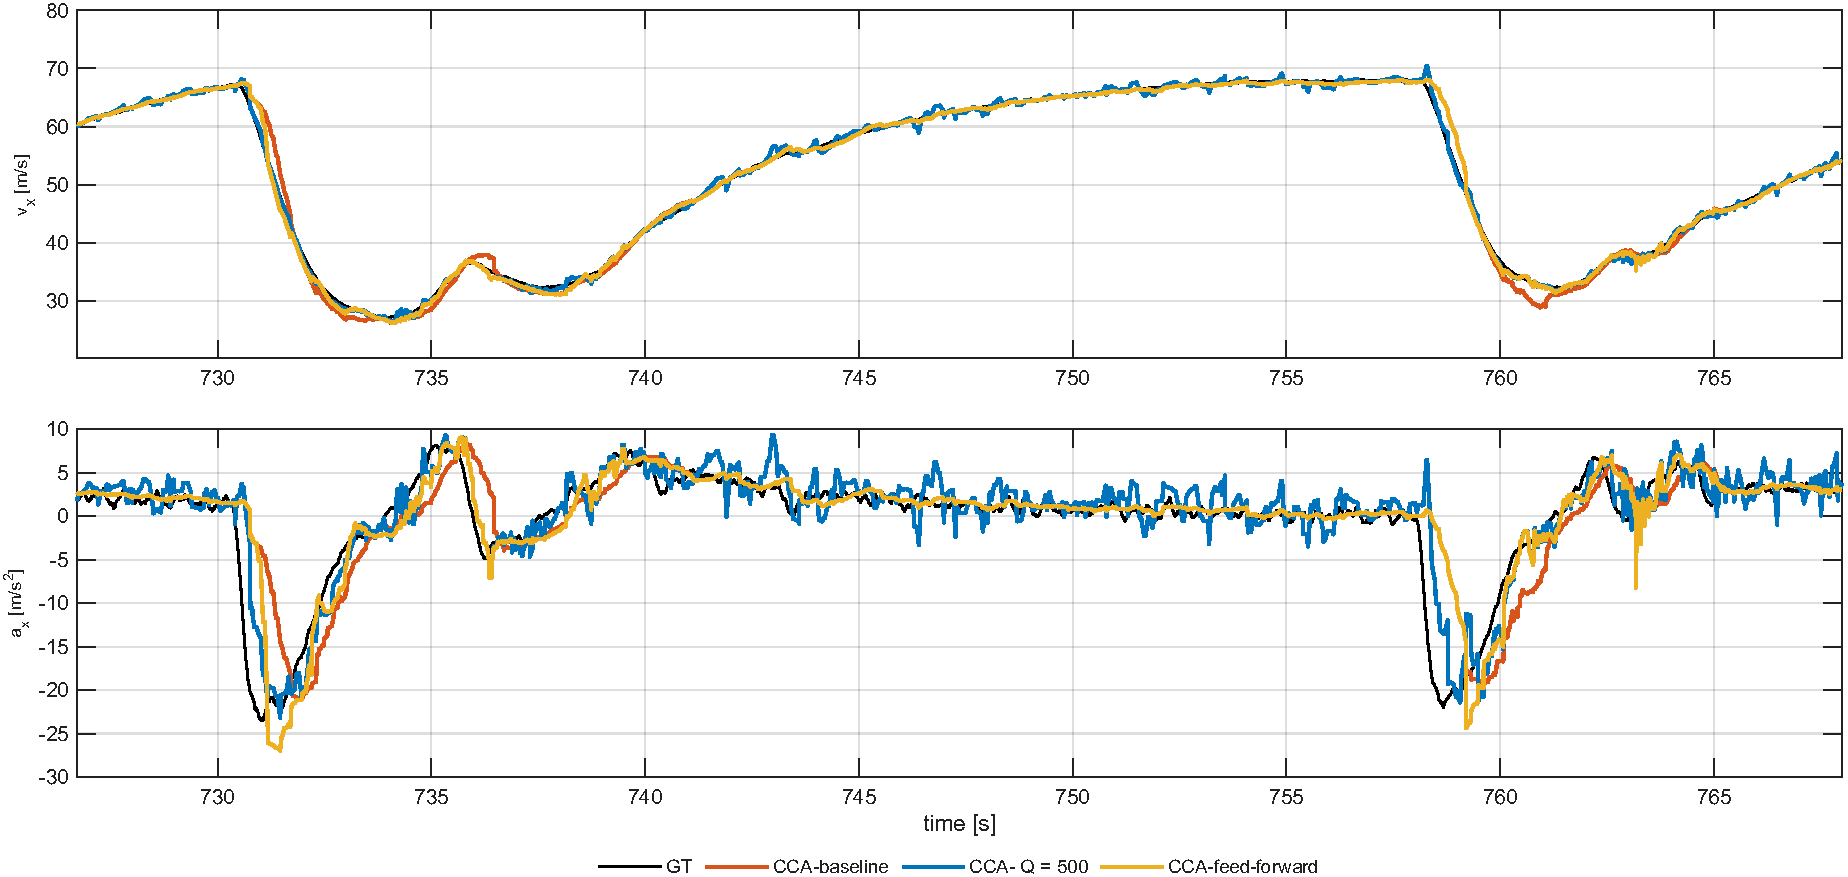
\includegraphics[width=\textwidth]{figures/ch5/qff_overview.pdf}
    \caption{Speed and acceleration estimated with the feed-forward process noise over a
    sequence of corners. Session of 5 September 2026, Imola.}
    \label{fig:qff_overview}
\end{figure}

Fig.~\ref{fig:qff_overview} shows the speed and the acceleration of the opponent over a
sequence that alternates braking phases with phases at almost constant speed. In the latter,
the estimate with the feed-forward process noise overlaps the nominal one and preserves its
smoothness, while the filter with the increased process noise follows the noise of the
measurements, which confirms that the flag remains inactive where the CCA model is adequate.
In the two braking phases between \SI{730}{s} and \SI{740}{s}, the flag is activated and the
feed-forward estimate approximates the ground truth better than the nominal filter, following
the drop of the acceleration earlier and with a smaller delay on the speed. The braking at
about \SI{760}{s}, instead, clearly shows the limit of the method. The flag is activated late,
when the deceleration is already in progress, so that during the braking the feed-forward
estimate accumulates the same delay as the nominal one, and it departs from it only in the
following phase of traction.

\begin{figure}[H]
    \centering
    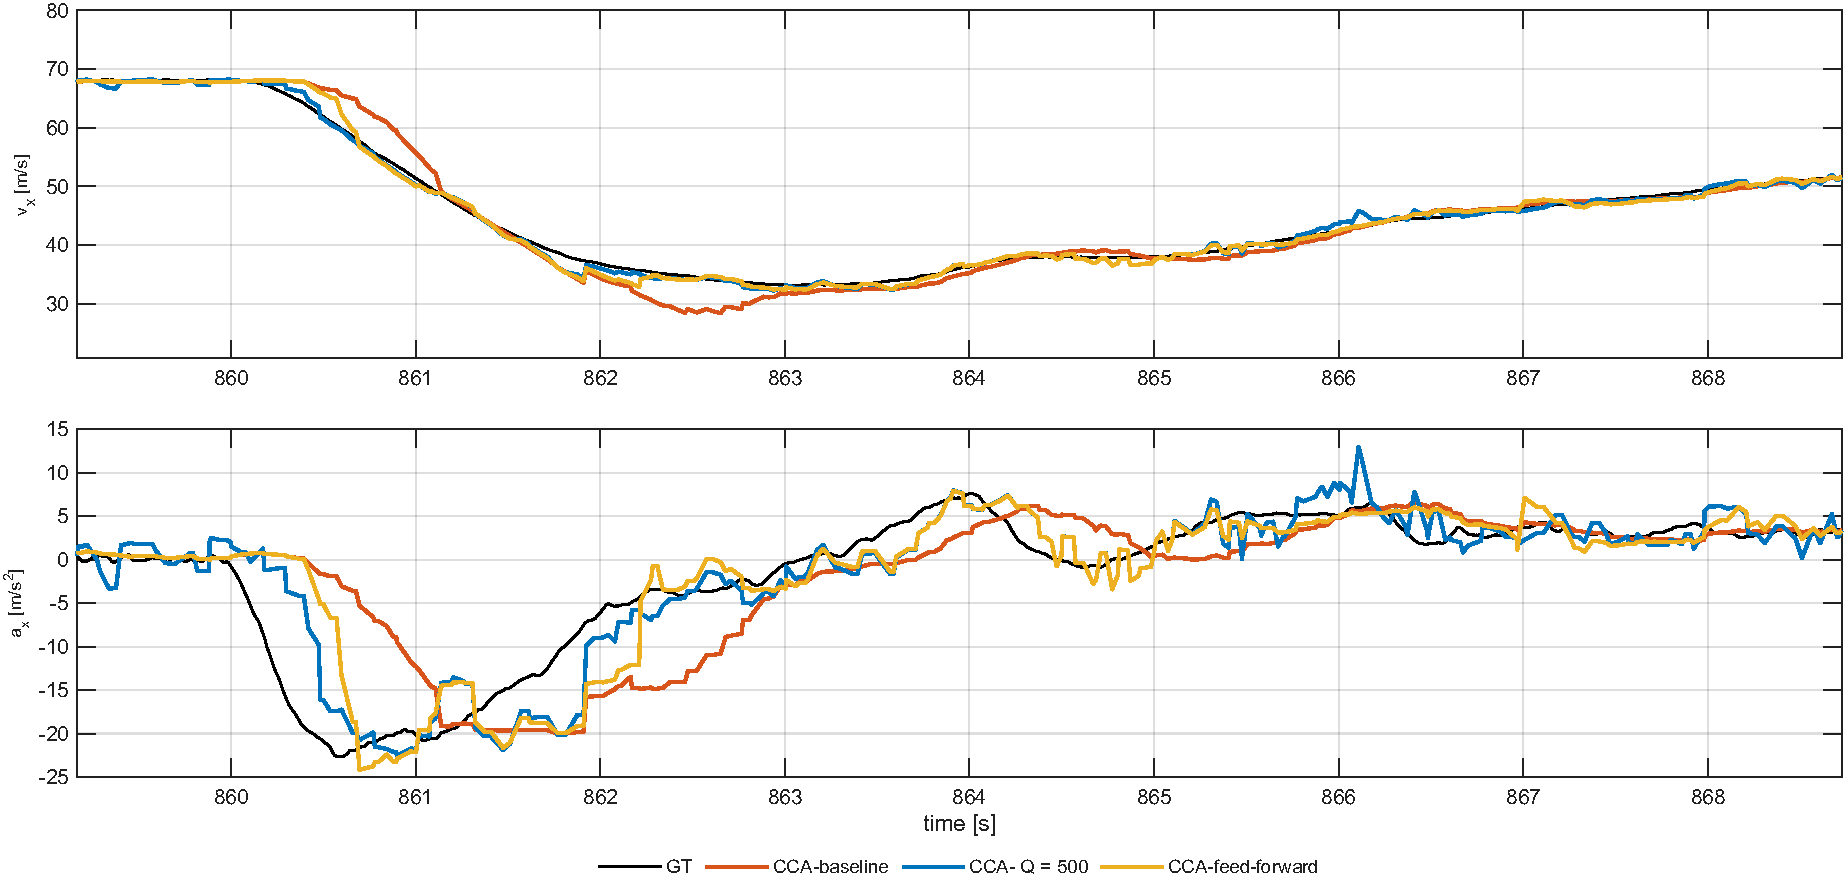
\includegraphics[width=\textwidth]{figures/ch5/qff_braking_detail.pdf}
    \caption{Detail of a braking phase. Session of 5 September 2026, Imola.}
    \label{fig:qff_braking_detail}
\end{figure}

The detail of Fig.~\ref{fig:qff_braking_detail} shows a braking in which the maneuver is
correctly detected. The feed-forward estimate starts to decrease with a slight delay with
respect to the filter with the increased process noise, but well before the nominal one,
whose delay is accumulated in the speed, which is underestimated at the end of the braking. The
feed-forward process noise therefore evidently improves the estimate of the nominal model, and
its speed remains close to the ground truth during the whole maneuver.

\begin{figure}[H]
    \centering
    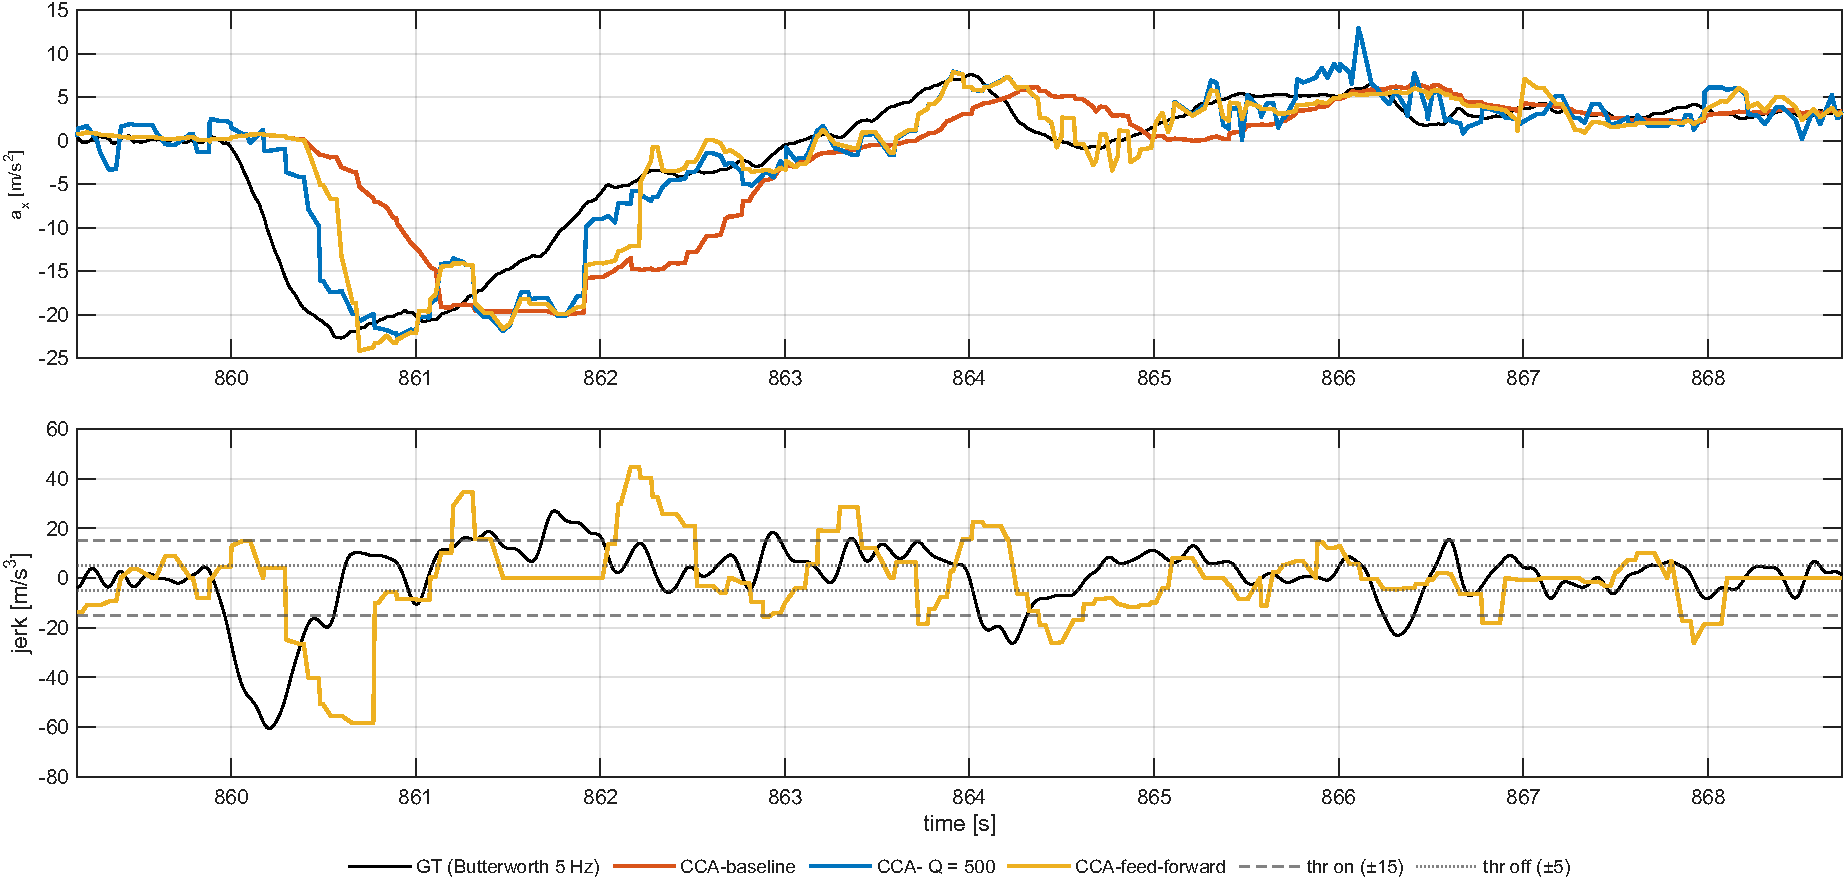
\includegraphics[width=\textwidth]{figures/ch5/qff_jerk.pdf}
    \caption{Acceleration and estimated jerk, with the activation thresholds of the flag, for
    the braking of Fig.~\ref{fig:qff_braking_detail}. Session of 5 September 2026, Imola.}
    \label{fig:qff_jerk}
\end{figure}

Fig.~\ref{fig:qff_jerk} complements Fig.~\ref{fig:qff_braking_detail} with the jerk estimated
from the auxiliary filter, compared with the jerk of the ground truth and with the thresholds
of the hysteresis. The estimated jerk detects the onset of the braking, but its main peak
follows the one of the ground truth with a slight delay, which is directly reflected on the
activation of the flag and explains the delay of the feed-forward estimate with respect to the
filter with the increased process noise. Moreover, in some intervals after the braking, the
estimated jerk exceeds the upper threshold while the jerk of the ground truth remains small,
causing spurious activations of the flag.

\begin{figure}[H]
    \centering
    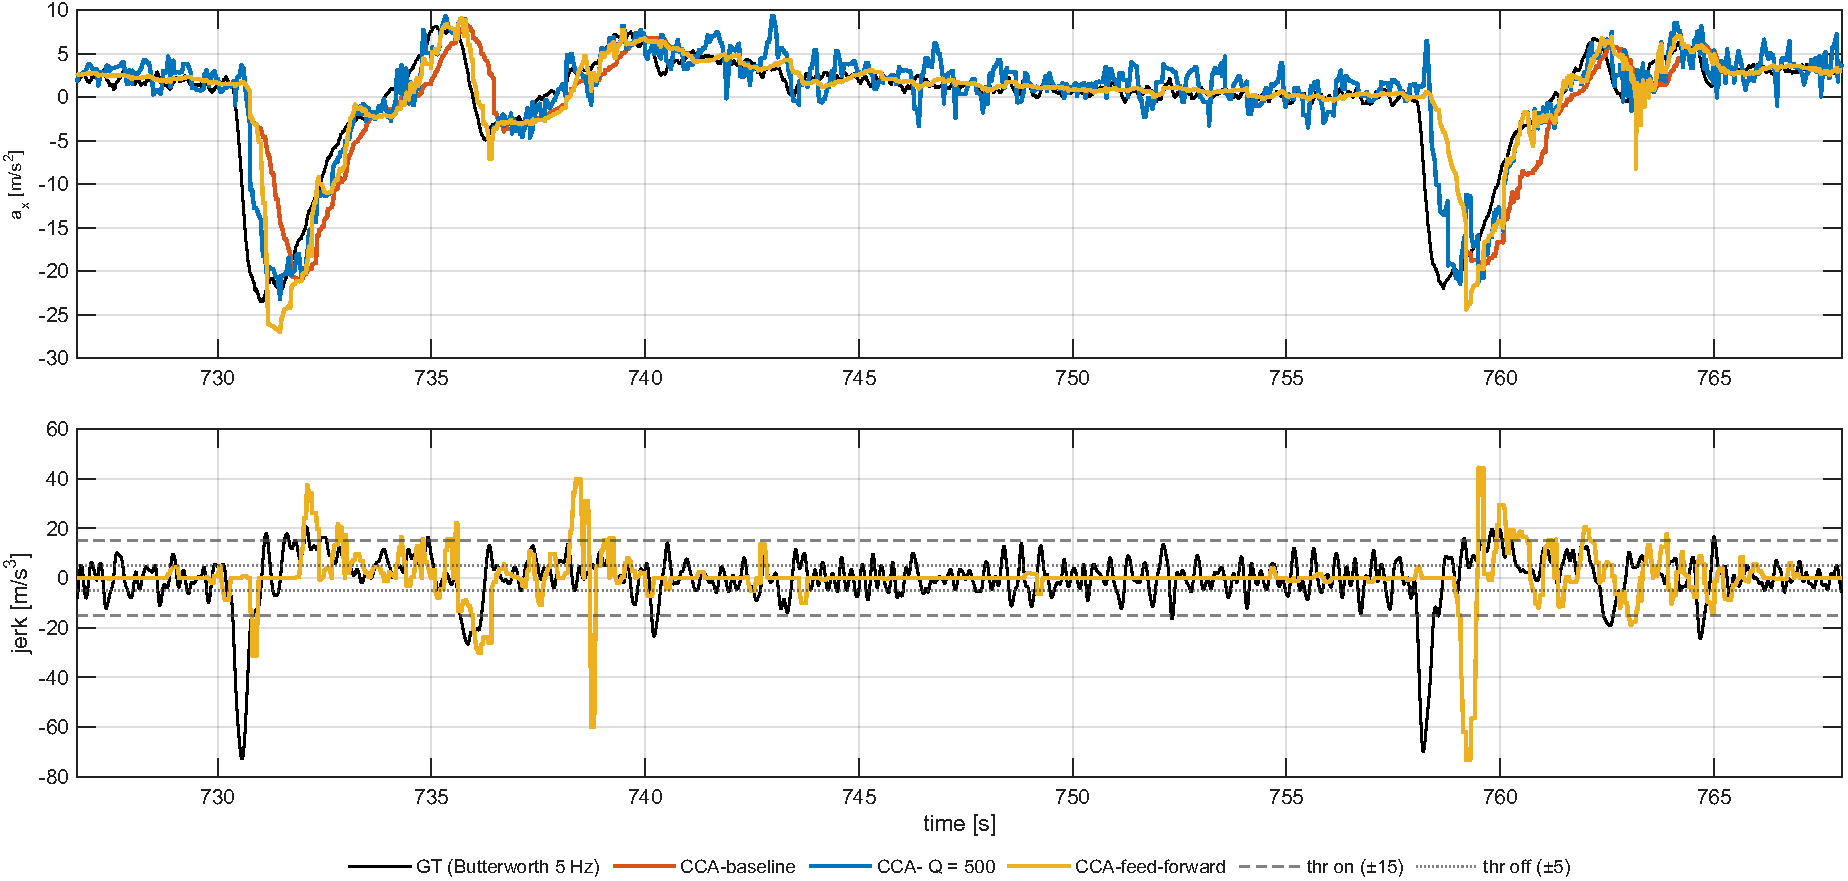
\includegraphics[width=\textwidth]{figures/ch5/qff_jerk_overview.pdf}
    \caption{Acceleration and estimated jerk, with the activation thresholds of the flag, for
    the maneuvers of Fig.~\ref{fig:qff_overview}. Session of 5 September 2026, Imola.}
    \label{fig:qff_jerk_overview}
\end{figure}

The same considerations hold for Fig.~\ref{fig:qff_jerk_overview}, which shows the jerk for
the maneuvers of Fig.~\ref{fig:qff_overview}. In particular, it shows the reason for the late
activation at about \SI{760}{s}. The jerk of the ground truth exhibits a sharp peak at the
onset of the braking, but the estimated jerk only reaches the upper threshold about one second
later, when the braking is already well developed, so that the delay of the feed-forward
estimate is entirely due to the delay of the estimator. Also in this case, isolated peaks of
the estimated jerk, e.g.\ at about \SI{739}{s}, exceed the thresholds while the jerk of the
ground truth remains small, leading to spurious activations.

Overall, the approach works and its principle is correct, since the flag remains inactive in
the phases at constant acceleration and is activated in the braking and traction phases, so
that the filter with the feed-forward process noise lies between the nominal filter and the one
with the increased process noise, keeping the smoothness of the former where the dynamics
changes slowly and approaching the reactivity of the latter during the maneuvers. The method,
however, presents limits related to the quality of the jerk estimator. Since the jerk is
ultimately obtained by differentiating the acceleration of the filter with the increased
process noise, it inherits the delay with which this filter follows the changes of the
dynamics, which is transferred to the activation of the flag, and the differentiation amplifies
part of its noise, which produces spurious activations also in phases in which the dynamics of
the opponent is not excited. In this perspective, the flag and its thresholds represent the
tuning knob of the method, since raising the activation threshold $j_{\mathrm{on}}$ reduces the
spurious activations but, at the same time, introduces a further delay in the activation when
an actual maneuver occurs.
